\documentclass[]{book}
\usepackage[english]{babel}
\usepackage{graphicx}
\usepackage{amsmath}
\usepackage{cite}
\usepackage{hyperref}


\begin{document}

\chapter*{Data Acquisition System }

\noindent La medición constituye un pilar fundamental de la investigación científica. Sin embargo, la cuantificación de una magnitud física solo se puede llevar a cabo a través de la interacción con el sistema y la extracción de la información de interés. A partir de estos conceptos es posible enmarcar la guía del presente capítulo, explorando los métodos que permiten convertir fenómenos físicos en señales que transporten información y las tecnologías que hacen posible la adquisición de dichas señales y su representación en un formato útil para el observador o  usuario \cite{webster2018measurement}. El conjunto de procesos diseñados para extraer información de un sistema físico se denomina sistema de adquisición de datos e incluye varias etapas que se ilustran en la figura \ref{fig:DAQ_generic} y se describen a continuación.\\

\begin{figure}[h]
    \centering
    
\includegraphics[width=1.0\textwidth]{DAQ_chain.png}
    \caption{Diagrama de los principales componentes de un sistema de adquisición de datos genérico}
    \label{fig:DAQ_generic}

\end{figure}

\noindent En primer lugar, es fundamental identificar un sistema de interés y las variables que se desean medir. Cualquier objeto físico puede ser estudiado siempre que se cuente con el marco teórico y los métodos experimentales adecuados para extraer sistemáticamente sus medidas. Por ejemplo, si se considera el universo observable, es posible medir su tasa de expansión mediante argumentos cosmológicos y un sistema de telescopios que observe cambios en las características de la luz proveniente de diversas galaxias, lo que evidencia la expansión del universo \cite{weinberg1976first}. Por otro lado, un tumor cerebral puede evaluarse al analizar los cambios en los espines nucleares de los átomos de hidrógeno en los tejidos cerebrales al aplicar un campo magnético potente para alinear estos espines, y luego pulsos de radiofrecuencia para perturbar esta alineación. La respuesta de los espines al campo magnético y a los pulsos de radiofrecuencia se detecta y se utiliza para crear imágenes detalladas de los tejidos cerebrales \cite{ernst1990principles}. Aunque estos ejemplos pueden parecer desconectados, comparten un elemento clave: son sistemas físicos cuyos atributos pueden medirse mediante la interacción con un medio capaz de extraer información. \\

\noindent El medio mencionado es diseñado sistemáticamente para interactuar con el objeto de interés. Estos medios son comúnmente dispositivos llamados sensores, un tipo de transductor capaz de convertir estímulos físicos en señales, generalmente eléctricas. Como se ha mencionado, existe una amplia variedad de sensores diseñados para medir todo tipo de magnitudes físicas, los cuales explotan distintos fenómenos en función de los requisitos de la medición \cite{webster2018measurement}. Por ejemplo, para medir la temperatura de un objeto, se pueden utilizar aleaciones metálicas que cambian su resistividad eléctrica ante variaciones de temperatura \cite{scarr1960thermistors}. Sin embargo, una cámara fotosensible al espectro infrarrojo también podría cumplir la misma función \cite{driggers2012introduction}. Estos sistemas se diferencian en la metodología con la que la información de los cambios de temperatura es transferida al usuario. En el primer caso, se requiere la lectura de la resistividad eléctrica y el conocimiento de su tasa de cambio en función de la temperatura, mientras que en el segundo caso, se emplea un sistema óptico equipado con la tecnología necesaria para convertir la radiación electromagnética en señales eléctricas. Finalmente estas señales pueden ser manipuladas para calcular la temperatura del objeto original utilizando la ley de Planck \cite{krane2019modern}.\\

\noindent Para lograr la extracción y transferencia efectiva de información hacia el observador, esta debe ser presentada en un formato que permita su codificación, transporte y almacenamiento sin pérdidas. En este contexto, las señales eléctricas, y por ende los dispositivos electrónicos, desempeñan un papel crucial en los sistemas modernos de adquisición de datos. Estos sistemas integran tanto componentes analógicos como digitales en sus diferentes etapas, tal como se ilustra en la figura \ref{fig:DAQ_generic}. \\

\noindent En general, las señales provenientes del sensor o detector deben ser tratadas y acondicionadas según las características que se deseen resaltar y preservar. Por ejemplo, es común que factores externos e internos de los sistemas electrónicos introduzcan señales no deseadas, conocidas como ruido, en la señal de interés, lo que hace necesario el uso de filtros de frecuencia o amplitud. Además, puede ocurrir que la señal generada por el sensor sea muy débil y las etapas subsecuentes no tengan la resolución adecuada para procesarla, por lo que se deben implementar amplificadores de distintos tipos. En otros casos, es necesario transformar el tipo de señal que transporta la información, por ejemplo, de carga a voltaje o de voltaje a corriente. Estas tareas suelen ser realizadas por circuitos de dispositivos analógicos, conocidos como etapas de acondicionamiento de señales, que algunos autores denominan analog front-end \cite{kledrowetz2023fully}.\\

\noindent Sin embargo, ante grandes volúmenes de datos, se requieren sistemas de cómputo con la capacidad de manejar señales con alta precisión, almacenar datos sin degradación y ejecutar operaciones complejas a gran velocidad, predominando los circuitos digitales como la tecnología principal en este ámbito. Como resultado, las etapas de procesamiento en los sistemas de adquisición de datos (DAQ) modernos están generalmente basadas en esta tecnología. Estos sistemas utilizan señales discretas, que representan información en forma de bits (0s y 1s), en contraste con las señales analógicas continuas. Como se mencionó anteriormente, estos sistemas aplican sobre las señales diversas operaciones, que pueden incluir clasificación, discriminación y la ejecución de operaciones matemáticas. Entre los principales exponentes de la electrónica digital se encuentran plataformas como procesadores o CPUs, FPGAs, ASICs, GPUs, DSPs, SoCs y computadoras cuánticas. Cada una de estas plataformas posee características únicas que las hacen especialmente adecuadas para diversas aplicaciones en el procesamiento de datos \cite{proakis2007digital}.\\

\noindent Si bien las plataformas mencionadas pueden ejecutar operaciones en linea, es decir, procesan las señales en la medida que ingresan al sistema, es necesario enviar la información a etapas externas del DAQ para llevar a cabo actividades como el almacenamiento, posprocesamiento, interacción con otros sistemas de detección (trigger) y transferencia a interfaces de alto nivel de abstracción como las computadoras de escritorio, para que el usuario pueda acceder a ella. Dependiendo de la complejidad de la aplicación y por ende del DAQ, distintos tipos de interfaces de comunicación pueden ser utilizados. Algunos ejemplos de estos protocolos, abarcando desde tecnología de consumo hasta grandes distribuciones de servidores son: RS-232, RS-485, USB, GPIB, Ethernet, Wi-Fi, Modbus/TCP, CAN Bus, Profibus, Profinet, SCADA, EtherCAT, MMS, MQTT, OPC UA, LHC Computing Grid, INFN-Tier-1 \cite{zurawski2014industrial} \cite{bortolotti2012infn}.\\

\noindent Finalmente, mediante el uso de programas informáticos diseñados específicamente para decodificar los datos provenientes de la interfaz de comunicación, las cantidades físicas de interés pueden presentarse en formatos comprensibles y útiles para el usuario. Por ejemplo, un osciloscopio que transmite datos a una computadora de escritorio a través de una interfaz GPIB-USB cuenta con una interfaz gráfica de usuario que permite visualizar la señal en el dominio del tiempo, destacando características como amplitud, frecuencia, y valor de la línea base. De manera similar, un sistema de espectroscopía nuclear puede enviar datos a través de Ethernet a un servidor, donde estos se almacenan en una base de datos accesible para usuarios de la red \cite{crespo2021remote}. Con aplicaciones web, es posible generar histogramas de energía frente a la altura, visualizando así los espectros de energía de una fuente de radiación. En última instancia, el objetivo de cualquier sistema de adquisición de datos, independientemente de su escala o infraestructura, es proporcionar al usuario información física relevante para su análisis e interpretación.\\

\noindent A continuación, se presentarán algunos conceptos clave sobre los sistemas de Adquisición de Datos (DAQ) con el propósito de profundizar en las características de sus etapas generales y establecer una base sólida para abordar el DAQ desarrollado en este trabajo. Posteriormente, se describirá el montaje experimental y la metodología empleada para su implementación.\\

\section{Marco Teórico}
\subsection{Sensores y Detectores}

\noindent Como se expuso anteriormente, un sensor es un dispositivo que detecta cambios en una cantidad física y los convierte en una señal que puede ser medida o interpretada. Formalmente, un sensor se define como un dispositivo que responde a un estímulo físico, químico o biológico específico, y genera una señal correspondiente, generalmente de tipo eléctrico, que tiene una relación funcional con la magnitud del estímulo. Los sensores suelen estar compuestos por dos componentes principales: el elemento sensible o transductor, que interactúa directamente con el estímulo (por ejemplo, temperatura, presión, luz, concentración química), y un mecanismo de conversión que traduce la respuesta del transductor en una señal utilizable (como una corriente o voltaje eléctrico). La precisión, sensibilidad, resolución y rango de operación son características clave que determinan el rendimiento de un sensor \cite{webster2018measurement}.\\

\noindent Los sensores se pueden clasificar según diversos criterios: por el tipo de magnitud que miden, el principio de funcionamiento (resistivos, capacitivos, inductivos, piezoeléctricos), el tipo de señal de salida (analógicos, digitales), la forma de operación (activos, pasivos), y la naturaleza del contacto con la magnitud medida (de contacto, sin contacto). Además, según su contexto de uso, los sensores pueden ser clasificados como domésticos (utilizados en electrodomésticos y dispositivos de consumo), industriales (empleados en automatización y control de procesos), o científicos (destinados a investigación y aplicaciones especializadas) \cite{sinclair2000sensors}.\\

\noindent En particular, estos últimos destacan por su alta precisión, exactitud, sensibilidad, robustez y fiabilidad. Su objetivo es proporcionar mediciones extremadamente precisas y reproducibles, ya que los resultados son cruciales para investigaciones avanzadas. Además, suelen poseer un amplio rango dinámico, lo que les permite detectar tanto variaciones muy pequeñas como extremadamente grandes en las magnitudes de interés. Un ejemplo destacado en este grupo son los detectores de radiación o partículas, que sobresalen por su capacidad para interactuar con corpúsculos a nivel atómico y subatómico, generando señales pulsadas que revelan propiedades esenciales de las partículas incidentes, como su energía, momento lineal o trayectoria, entre otras \cite{kolanoski2020particle}.

\subsection{Señales Eléctricas de Sensores}

\noindent Dado que las señales eléctricas son esenciales en este contexto como portadoras de la información física que se busca extraer, es fundamental describir sus principales características para comprender cómo las etapas electrónicas del sistema de adquisición de datos (DAQ) las afectan. Aunque las señales pueden ser digitales o análogas, generalmente las producidas por un sensor o detector son de tipo análogo. \\

\noindent Una señal analógica proveniente de un sensor se caracteriza principalmente por su variación continua en el tiempo y su capacidad para representar información en un rango infinito de valores. La amplitud de la señal refleja la magnitud del parámetro medido, como temperatura o presión, y puede variar suavemente en respuesta a cambios en el entorno. La frecuencia de la señal puede no ser relevante en todos los casos, pero el tiempo de respuesta y la estabilidad son cruciales para asegurar mediciones precisas. Además, la señal puede estar afectada por ruido y errores, lo que requiere técnicas de filtrado y calibración para obtener datos confiables. La forma de onda de la señal es continua y puede ser analizada en el dominio del tiempo para evaluar su comportamiento y en el dominio de la frecuencia para identificar componentes relevantes \cite{sinclair2000sensors}. En la figura \ref{fig:generic_signal}, se ilustra una señal en el dominio del tiempo proveniente de un sensor de aceleración

\begin{figure}[h]
    \centering
    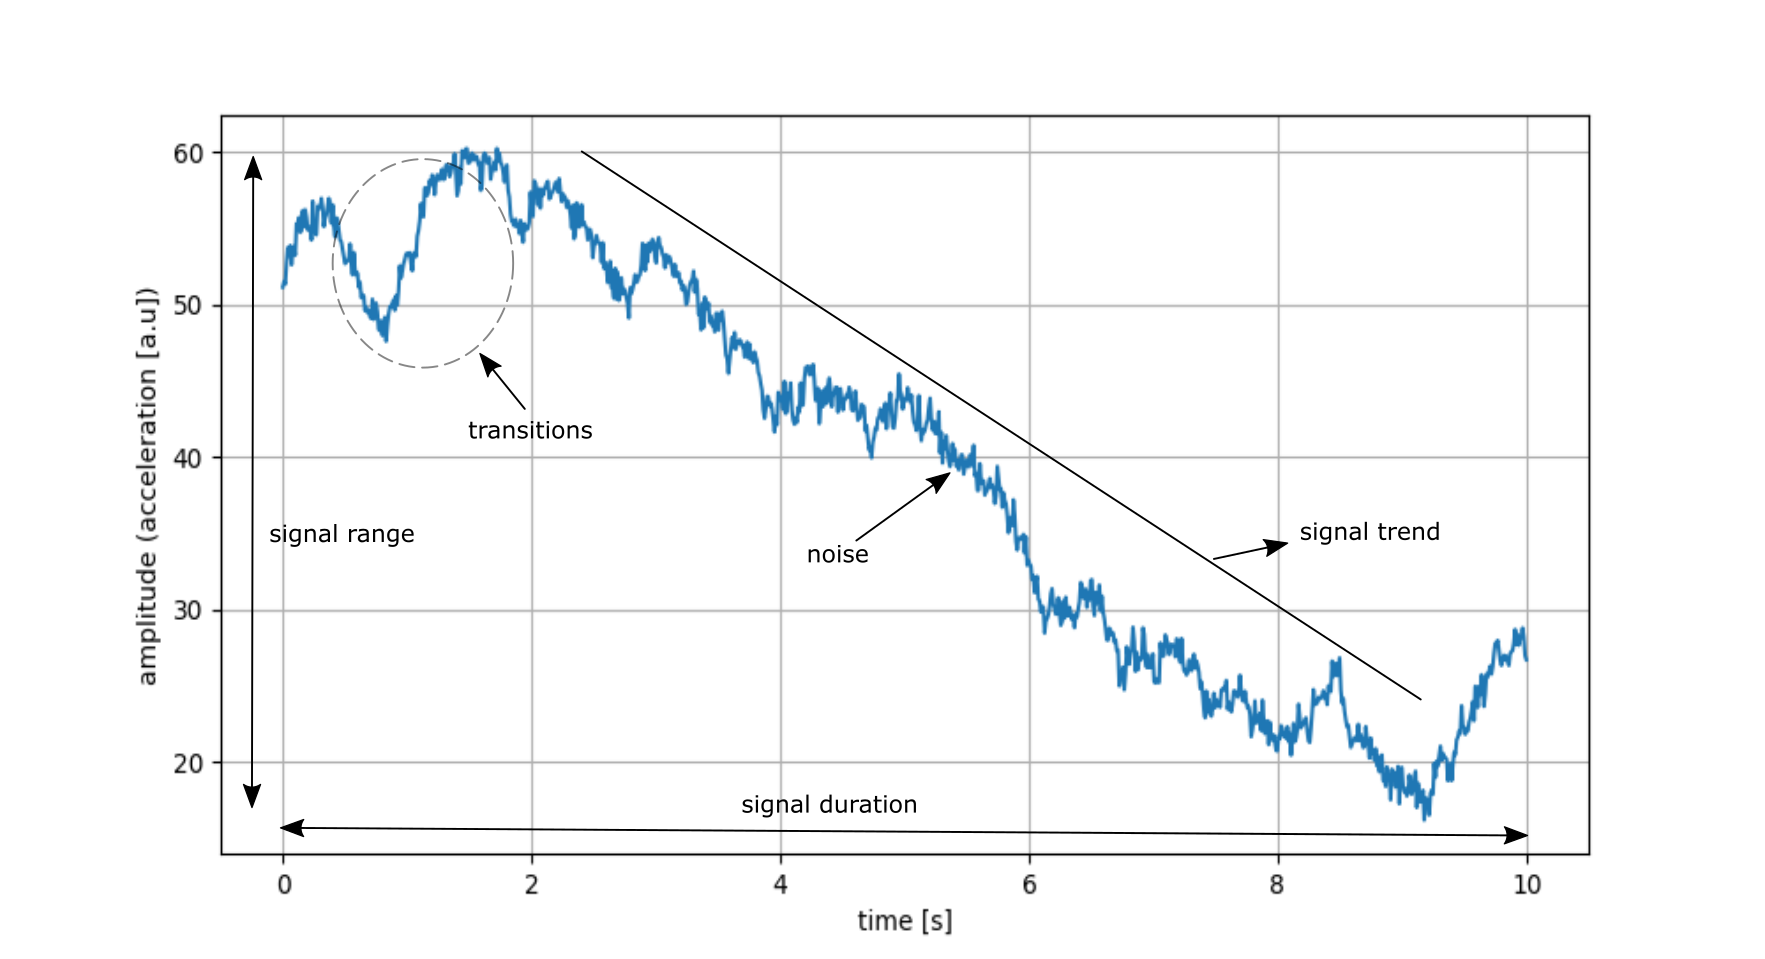
\includegraphics[width=0.8\textwidth]{mysignal.png}
    \caption{Señal no periódica en el dominio del tiempo proveniente de un sensor de aceleración. En ella es posible observar algunas características como duración, rango de la magnitud de interés en el lapso registrado, ruido electrónico, tendencia y transitorios. La amplitud de la señal solo puede ser definida con base a un nivel de referencia.}
    \label{fig:generic_signal}

\end{figure}

\noindent Un caso de particular interés son las señales producidas por los detectores de partículas, que en general son de naturaleza pulsada. En este contexto, se puede asociar la detección de un evento con una perturbación, denominada pulso, que se define sobre la línea base de la señal de salida. La figura \ref{fig:pulse} muestra un ejemplo genérico de un pulso individual, utilizado para ilustrar algunas de sus características principales.\\

\begin{figure}[h]
    \centering
    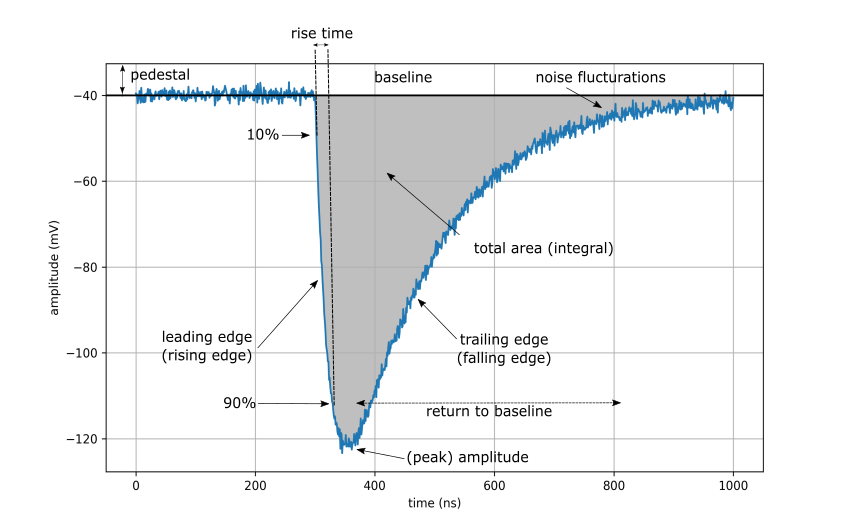
\includegraphics[width=1.0\textwidth]{pulse_edited.png}
    \caption{Pulso típico genérico para ilustrar las principales características. Reproducido a partir de \cite{kolanoski2020particle}}
    \label{fig:pulse}

\end{figure}

\noindent Según \cite{knoll2010radiation}, suponiendo que la señal generada por el detector es corta comparado con los tiempos típicos de procesamiento de la electrónica de lectura, las cantidades que caracterizan un pulso son:

\begin{itemize}
    \item La amplitud máxima del pulso: también conocida como altura del pulso, es el valor máximo que alcanza la señal. En sistemas lineales, este valor es proporcional a la energía primaria depositada en el detector.
    \item Tiempo de pico: Es el momento en el tiempo en el que se alcanza la amplitud máxima del pulso.
    \item Área o integral del pulso: Representa el área bajo la curva del pulso. En sistemas lineales y para señales cortas tipo $\delta$, su valor debería ser proporcional a la energía primaria depositada.
    \item Ancho del pulso: Se refiere a la duración del pulso, que generalmente se define como el ancho total a la mitad de la altura máxima (FWHM, por sus siglas en inglés).
    \item Bordes de subida y bajada: Son las pendientes ascendente y descendente del pulso.
    \item Tiempo de subida: Caracteriza la rapidez con la que el pulso aumenta. Comúnmente se define como el tiempo necesario para que el pulso pase del 10\% al 90\% de su amplitud máxima, aunque existen otras definiciones.
    \item Tasa de variación (Slew rate): Indica el cambio de voltaje por unidad de tiempo $dV/dt$ y se expresa en unidades de $V/s$.
    \item Línea base o valor de pedestal: Es el valor de salida cuando no hay ninguna señal de entrada. Define el nivel 'cero' desde el cual se mide la altura de la señal. Aunque generalmente la línea base tiene un valor fijo, pueden ocurrir desviaciones durante un cierto (y breve) período de tiempo. Estas desviaciones se conocen como desplazamientos de la línea base.
    \item Tiempo de retorno a la línea base: Es el tiempo necesario para que la amplitud del pulso vuelva al valor de la línea base.
    \item Suboscilación: Se refiere a la parte de la amplitud de un pulso que tiene un signo opuesto (con respecto a la línea base) en comparación con la amplitud principal.
    \item Señal unipolar: Es una forma de pulso en la que, salvo por las fluctuaciones de ruido, el valor de la amplitud se mantiene por encima o por debajo de la línea base en todo momento $t$. Por lo general, también se incluyen en esta definición las señales con pequeñas suboscilaciones.
    \item Señal bipolar: Es una forma de pulso en la que la parte del pulso que ocurre más tarde en el tiempo tiene un signo opuesto al de la parte que ocurre primero.
\end{itemize}

\noindent Por otro lado, las señales digitales, esenciales en el procesamiento de información, se caracterizan por su naturaleza discreta tanto en el tiempo como en la amplitud. Estas señales solo pueden adoptar dos estados, representados por los valores 1 y 0. A partir de una señal base con frecuencia constante, conocida como reloj, se puede codificar información en señales digitales mediante código binario y operaciones de conteo. Básicamente, se mide cuántos ciclos de reloj la señal permanece en un estado u otro. Esta metodología es altamente versátil, ya que permite realizar operaciones matemáticas utilizando el sistema binario \cite{brown2000fundamentals}.

\begin{figure}[h]
    \centering
    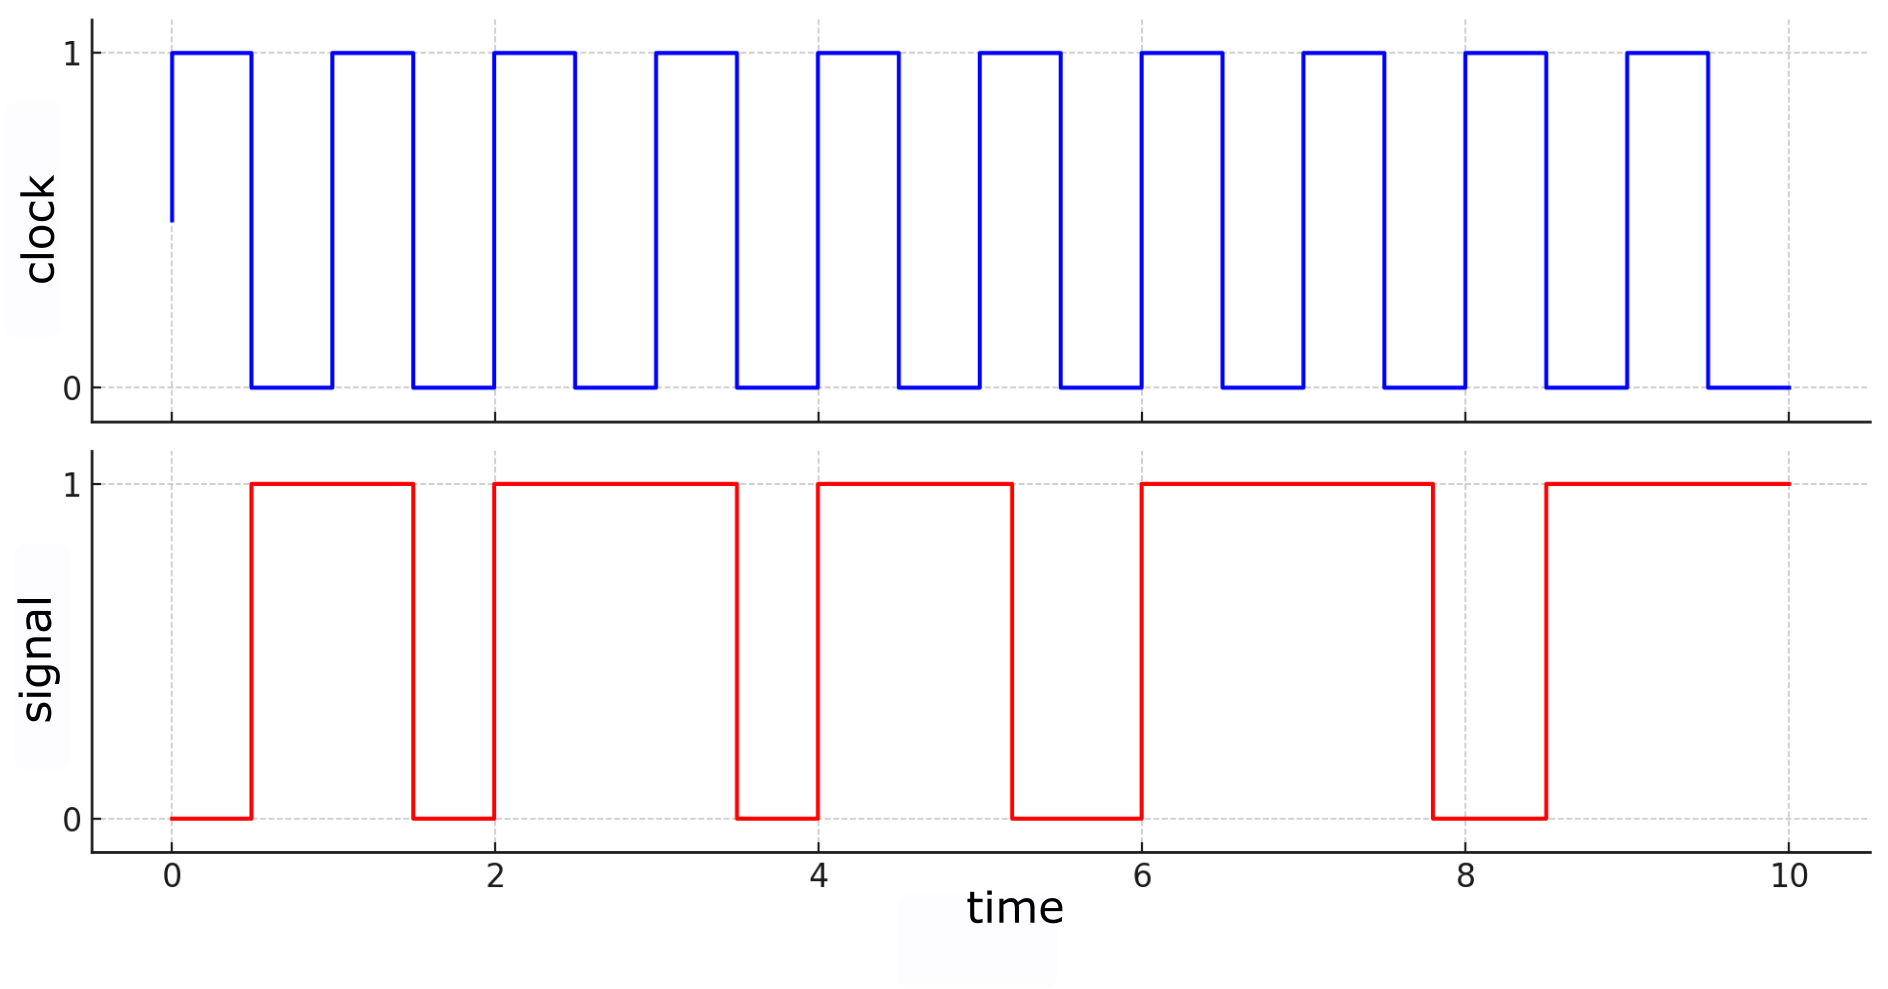
\includegraphics[width=0.7\textwidth]{digital_signal.png}
    \caption{Señal digital}
    \label{fig:digital_siganl}

\end{figure}

\section{Tratamiento y acondicionamiento de Señales}

\noindent Próxima al detector, se encuentra la etapa denominada front-end, que típicamente comprende electrónica analógica para la amplificación de la señal, shaping y discriminación, así como digitalización y transporte. A continuación pueden encontrarse sistemas de más alto nivel como procesadores digitales y de adquisición de datos, que permiten transformar las señales y extraer la información necesaria para su posterior estudio. En la figura \ref{fig:generic_frontend} se observa un esquema genérico de la electrónica de front-end de un detector.\\

\begin{figure}[h]
    \centering
    
\includegraphics[width=0.8\textwidth]{front-end.png}
    \caption{Un esquema de electrónica de front-end típico, utilizado a menudo para la lectura de un
    detector, que incluye amplificación, conformación de impulsos y digitalización (representada aquí por un ADC).}
    \label{fig:generic_frontend}

\end{figure}

\noindent Los sistemas involucrados en la electrónica de front-end, deben cumplir con tres características: (a) ser causales, (b) invariantes en el tiempo, y (c) lineales al menos en la primera etapa de amplificación. Un sistema se considera causal si, en cualquier momento, solo depende del valor de su entrada en ese instante. Es invariante en el tiempo si la relación entre la salida y la entrada, por ejemplo, el ratio $\text{señal}_{\text{entrada}}/\text{señal}_{\text{salida}}$ no varía con el tiempo \cite{kolanoski2020particle}. La linealidad del sistema implica que el pulso de salida (por ejemplo, $v_{out(t)}$) no depende del tamaño de la señal de entrada (por ejemplo, $i_{in(t)}$), esto es, 

$$
v_{\text {out }}\left(\alpha \times i_{\text {in }}(t)\right)=\alpha \times v_{\text {out }}\left(i_{\text {in }}(t)\right)
$$

\noindent Tal es el caso de los detectores GEM. Las corrientes típicas medidas en su salida pueden ser muy pequeñas, del orden de nanoamperios [citar]. Por lo tanto, es necesario implementar etapas de preamplificación y amplificación, hasta lograr señales con características adecuadas para su digitalización y el subsecuente procesamiento. Sin embargo, si se busca procesar señales de voltaje, es necesario conectar una resistencia $R$ en serie con la salida del detector para medir una señal de voltaje $V$ en sus terminales, de acuerdo a la ley de Ohm, $$V = R I$$ 

\subsubsection{Preamplificador}

\noindent Como expone \cite{knoll2010radiation}, La función principal del preamplificador es captar la señal del detector sin deteriorar notablemente la SNR inherente. Por ello, el preamplificador se ubica generalmente lo más cerca posible del detector para reducir la carga capacitiva $(C)$ sobre este. El preamplificador de voltaje amplifica directamente la señal de voltaje $V_{\text{in}}$, manteniendo una alta impedancia de entrada $Z_{\text{in}}$ y una baja impedancia de salida $Z_{\text{out}}$ para asegurar una transferencia eficiente y reducir la influencia del ruido. En ambos casos, la linealidad del preamplificador es crucial para que la relación $V_{\text{out}}/ V_{\text{in}}$ se mantenga constante, lo cual es esencial para la precisión en la medición \cite{leo1994techniques}.\\

\noindent Por otro lado, un preamplificador de carga convierte una señal de carga $Q$ generada por el detector en un voltaje proporcional $V$, dada la relación: $$V = \frac{Q}{C}$$ La figura \ref{fig:preamp} ilustra su comportamiento típico sobre la señal del detector.\\

\begin{figure}[h]
    \centering
    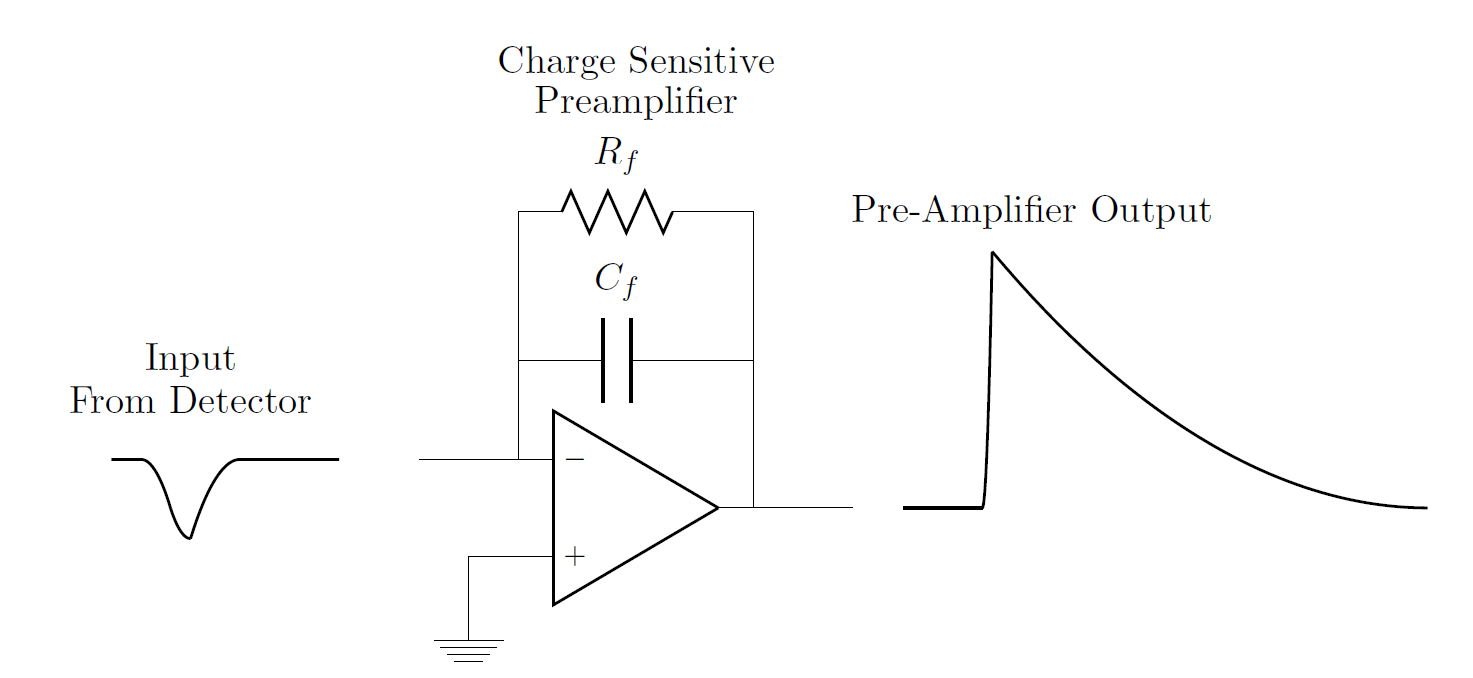
\includegraphics[width=0.8\textwidth]{preamp.PNG}
    \caption{Ilustración del comportamiento típico del preamplificador de carga.}
    \label{fig:preamp}

\end{figure}

\noindent Como explica \cite{proakis2007digital}, la amplificación por etapas de una señal ofrece numerosas ventajas significativas. Principalmente, permite reducir el ruido generado en cada etapa individual, resultando en una señal final más limpia y menos propensa a la distorsión. Este método también mejora la estabilidad del sistema al distribuir la amplificación, evitando la saturación que podría ocurrir con una amplificación intensa en una sola etapa. Además, facilita el control preciso de la ganancia y la adaptación de impedancias entre diferentes componentes, lo cual mejora la eficiencia y la transferencia de la señal. La amplificación gradual es particularmente útil para manejar señales débiles, amplificándolas sin riesgo de distorsión. Asimismo, distribuye la carga térmica generada, disminuyendo el riesgo de sobrecalentamiento de los componentes. \\

\subsubsection{Amplificador}

\noindent En general, se realiza mediante un amplificador operacional con una resistencia en realimentación. Como modelo matemático, el detector, representado como una capacitancia a descargar, suministra la señal de corriente $i_{s}$ a través de la resistencia $R_{s}$ a un nivel de referencia en un tiempo $\Delta t$. Si el tiempo de descarga es grande comparado al tiempo de duración de la señal $$\left(\tau=R_S C_D \gg\right. \Delta t)$$ en cierto sentido, el detector integra la señal de corriente en la capacitancia del detector $$\left(V_D=Q_S / C_D\right)$$ y a la entrada del amplificador se tiene el voltaje $$v_{\text{in}}(t)=V_D \exp \left(-t / R_S C_D\right)$$ El voltaje de salida es proporcional a $v_{i n}$ y el sistema opera como un amplificador de voltaje [1]:
$$
v_{\text {out }}(t)=-\frac{R_f}{R_S} v_{\text {in }}(t)=-\frac{R_f V_D}{R_S} \exp \left(-t / R_S C_D\right) .
$$

\subsubsection{Signal Shaping}

\noindent En la cadena de modulación de señales de la electrónica de front-end, la etapa de shaping es un circuito electrónico diseñado para modificar la forma de una señal de pulso para mejorar su calidad y adecuarla a las necesidades de procesamiento posterior. Está encargado de transformar las señales pulsadas del detector, que pueden tener formas variadas, en pulsos uniformes y bien definidos. Esto es crucial para evitar la superposición de pulsos (pile-up) y reducir el ruido mediante filtrado de frecuencia \cite{leo1994techniques}.\\

\noindent Los pulsos electrónicos generados por el preamplificador tienen tiempos de decaimiento típicos que varían entre unos pocos nanosegundos y varios microsegundos. Si llegan señales adicionales durante el tiempo de decaimiento, puede ocurrir pile-up a pesar de que el capacitor de retroalimentación del preamplificador se descargue. Para mitigar esto, se utilizan filtros pasa-altos y pasa-bajos, que permiten separar las señales superpuestas y moldear los pulsos de salida en formas más Gaussianas. Además, los filtros ayudan a reducir el ruido blanco que afecta a todas las frecuencias, mejorando así la SNR \cite{kolanoski2020particle}.\\

\subsubsection{Digitalización}

\noindent De acuerdo a \cite{knoll2010radiation}, la digitalización de las señales provenientes de un detector es crucial debido a la precisión y flexibilidad que ofrece frente a los métodos analógicos tradicionales. Con el avance de los convertidores analógico-digitales (ADC) de alta velocidad y buena resolución desde los años 90, la posibilidad de procesar digitalmente los pulsos de los detectores se ha consolidado.\\

\noindent Las ventajas de este enfoque incluyen una flexibilidad ilimitada en la elección de parámetros de conformación, mayor estabilidad al eliminar el riesgo de derivas debido a cambios de temperatura o voltaje, y la capacidad de realizar análisis más detallados con múltiples salidas de un mismo detector. Además, la manipulación digital no introduce ruido adicional y permite la implementación precisa de formas de pulso que serían difíciles o imposibles de lograr en circuitos analógicos. Sin embargo, una desventaja potencial es la limitación en la precisión del tiempo de detección, ya que los sistemas digitales están restringidos a la frecuencia de muestreo más cercana, lo que puede ser menos exacto que los métodos analógicos simples en aplicaciones que requieren una temporización muy rápida.\\

\noindent La función principal de un ADC es generar un código digital o número en su salida, que sea proporcional a la tensión analógica suministrada a su entrada. En un ADC genérico, las conversiones se realizan de forma continua a una frecuencia de reloj fija. Por ejemplo, un reloj de 500 MHz producirá 500 MSPS (Megasamples per Second), lo que equivale a una muestra cada 2 ns. \\

\noindent Un número binario con $n$ bits puede representar $2^{n}$ valores. Durante la digitalización, el rango de voltaje desde $V_{\text{min}}$ (usualmente $V_{\text{min}} = 0$) hasta $V_{\text{max}}$ se subdivide en $2^{n} - 1$ intervalos, a cada uno de los cuales se le asigna un valor binario. Si la conversión es lineal, el rango se divide en intervalos de tamaño igual. El paso de voltaje más pequeño corresponde al bit menos significativo (LSB, por sus siglas en inglés), que se encuentra más a la derecha en un número binario. En un convertidor analógico-digital (ADC) de $n$ bits, un LSB corresponde a un paso de voltaje de:

$$
1 \text{ LSB} = \frac{V_{\text{max}} - V_{\text{min}}}{2^n - 1}
$$

\noindent En un ADC ideal, cada conversión de voltaje de entrada a código de salida es independiente, perfectamente lineal y ocurre instantáneamente. Sin embargo, las imperfecciones en los ADCs reales limitan tanto la frecuencia máxima de muestreo como la linealidad y la precisión de la conversión \cite{kolanoski2020particle}. 

%incluir fotografía de la tarjeta

\section{DAQ and Digital Processing}

\noindent Si bien existen diversos tipos de hardware programable para el despliegue de sistemas embebidos como los microcontroladores y procesadores, en función de los requerimientos impuestos por un ADC de alta velocidad y la necesidad de contar con una plataforma flexible para la evolución de un sistema de detección experimental, es necesaria la implementación de un dispositivo basado en FPGA. En la figura \ref{fig:pulse_chain} se ilustra la ubicación típica de la plataforma digital de procesamiento en la cadena de lectura de un detector.
%quitar la parte de acondicionamiento y dejar solo la digital
\begin{figure}[h]
    \centering
    
\includegraphics[width=0.8\textwidth]{pulse_chain_generic.png}
    \caption{Un esquema de la cadena de electrónica usualmente utilizado para la lectura de un
    detector, que ilustra la etapa de adquisición y procesamiento digital a continuación de la etapa de front-end.}
    \label{fig:pulse_chain}

\end{figure}

\subsubsection{FPGA}
\noindent Una FPGA es un tipo de circuito integrado reconfigurable que permite a los usuarios personalizar su arquitectura interna para realizar tareas específicas, lo que las diferencia de los microprocesadores tradicionales que siguen un conjunto de instrucciones fijas. Estas matrices de puertas programables en campo son ampliamente utilizadas en aplicaciones que requieren procesamiento en paralelo y alta flexibilidad, como en sistemas de telecomunicaciones y procesamiento de señales digitales. \\

\noindent La capacidad de ser reprogramadas múltiples veces les otorga una ventaja significativa en términos de adaptabilidad a nuevas necesidades sin requerir cambios físicos en el hardware. Para programar una FPGA, se emplean lenguajes de descripción de hardware (HDL), como VHDL o Verilog, lo que permite definir circuitos personalizados que se cargan directamente en el dispositivo, haciendo que se comporten según el diseño especificado \cite{brown2000fundamentals}.\\

\noindent Este tipo de arquitectura ofrece baja latencia, lo cual es esencial para manejar el alto volumen de datos generados por los ADCs de alta velocidad. Además, su capacidad de procesamiento paralelo permite el manejo eficiente de altas tasas de muestreo, asegurando que los datos provenientes del detector se procesen minimizando la pérdida de información. En particular, las FPGA proporcionan una flexibilidad considerable en el diseño y la implementación de algoritmos de procesamiento de señales, contando con módulos de hardware dedicado a esta tarea llamados DSP (Digital Signal Processor) \cite{meyer2007digital}.\\

\subsubsection{FPGA SoC}

\noindent No obstante, como expone \cite{bravo2020new}, los avances en tecnología FPGA se han direccionado al desarrollo de sistemas híbridos como los SoC. De acuerdo a \cite{amd_zynq_7000}, Un FPGA SoC es un dispositivo que combina en un solo chip la flexibilidad programable de una FPGA, también denominado PL (Programmable Logic), con las capacidades de procesamiento de un procesador o PS (Processing System), típicamente basado en la arquitectura ARM. La figura \ref{fig:fpga_soc} ilustra la infraestructura típica de un SoC. \\ 

\noindent Esta configuración permite aprovechar lo mejor de ambos mundos: la capacidad de realizar tareas complejas y variables mediante software y, al mismo tiempo, la ejecución de operaciones intensivas en paralelo y en tiempo real mediante la lógica programable de la FPGA. Además, esta integración incluye funcionalidades adicionales como procesamiento digital de señales (DSP), dispositivos de señal mixta, y la posibilidad de reemplazar otros componentes dedicados como los ASICs (Application-Specific Integrated Circuits) o ASSPs (Application-Specific Standard Products), todo en un solo dispositivo, optimizando así el rendimiento y la eficiencia energética para aplicaciones específicas.\\

\begin{figure}[h]
    \centering
    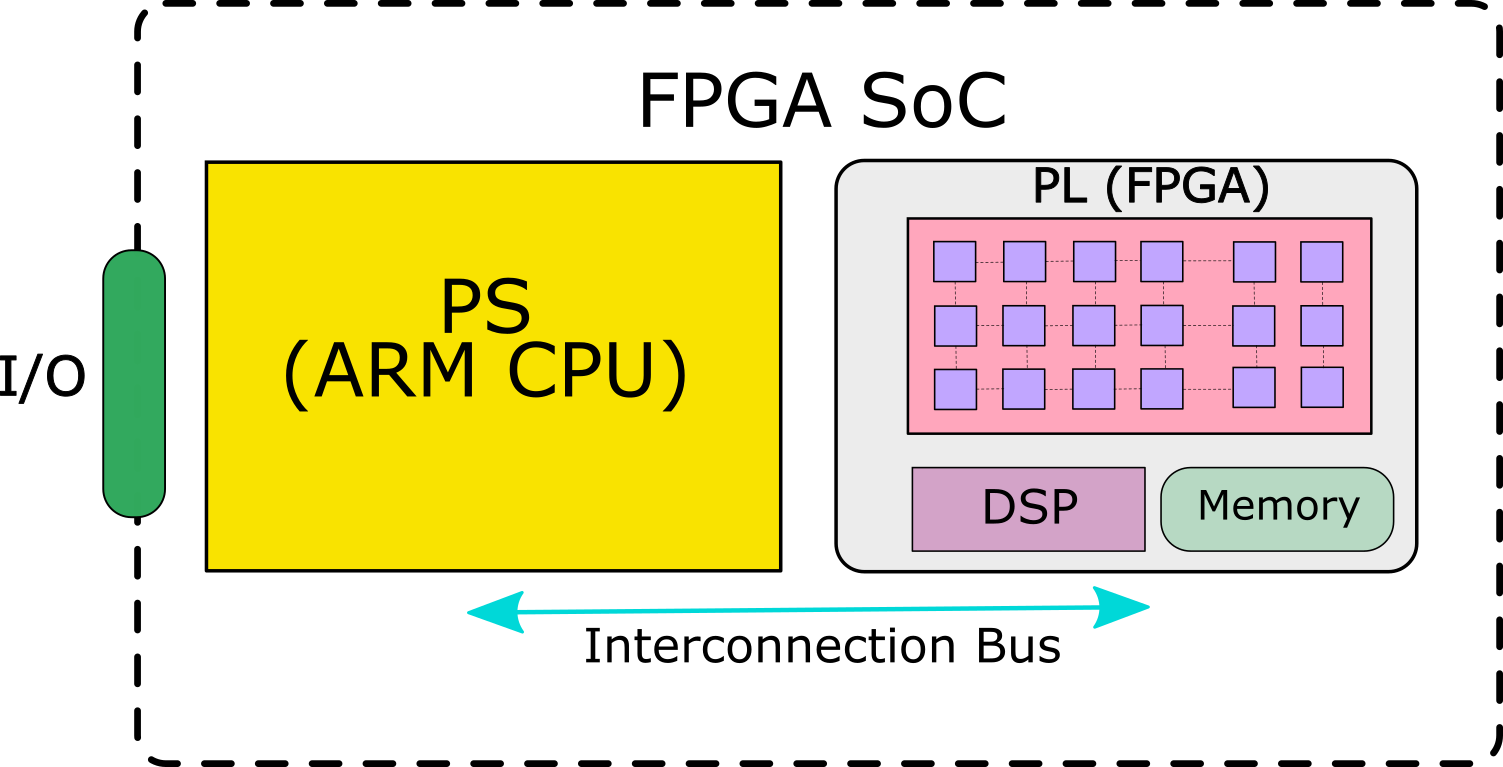
\includegraphics[width=0.6\textwidth]{FPGA_SoC.png}
    \caption{Arquitectura típica de un FPGA SoC.}
    \label{fig:fpga_soc}

\end{figure}

\subsection{Procesamiento Digital de Pulsos}
 
\noindent Como se explicó en el apartado de electrónica de front-end, los filtros analógicos suelen aplicar una combinación de diferenciaciones e integraciones de la forma de onda de voltaje para transformarla en una forma similar a la de una gaussiana, cuya amplitud es proporcional al voltaje $V$ y, por lo tanto, a la energía de la radiación. Sin embargo, de acuerdo a \cite{loudenuclearspectroscopy}, en el enfoque digital, tras la digitalización de la señal utilizando un ADC, se aplica un filtro matemático a esta serie de valores digitales para eliminar los componentes de ruido de alta frecuencia, mejorando así la SNR y determinando la amplitud de voltaje $V$.\\

\noindent Este enfoque presenta ventajas significativas en comparación con el procesamiento de señales analógicas tradicional, entre las cuales destacan \cite{radeka1968optimum}:

\begin{itemize}
    \item Aplicación de análisis considerando diferencias pulso a pulso: Permite analizar cada pulso individualmente, teniendo en cuenta sus particularidades.
    \item Análisis de señales de carga inducida transitoria: Facilita la interpretación de señales transitorias que pueden ser difíciles de captar con métodos analógicos.
    \item  Mejora del parámetro de tiempo muerto: Reduce las limitaciones temporales que pueden afectar la adquisición continua de señales.
    \item Captura fácil de señales, incluida la implementación de análisis complejos: Simplifica la adquisición de datos y permite realizar análisis detallados y sofisticados.
    \item Procesamiento de señales con criterios basados en coincidencias (diferentes detectores o diferentes partes del mismo detector): Facilita la correlación de eventos entre múltiples detectores o áreas de un detector.
    \item Aplicación efectiva de post-procesamiento de datos: Permite el pre-análisis de formas de onda, modelado de pulsos y verificación de algoritmos de deconvolución de superposición de pulsos (pulse pile-up).

\end{itemize}

\noindent La implementación de procesadores digitales de pulsos (DPP) en FPGA, gracias a su riqueza en recursos lógicos digitales, les permite soportar múltiples modos de adquisición, como análisis de altura de pulso, escalado de canales múltiples, escalado de espectros múltiples y adquisición en modo de lista con marcas de tiempo. Además, ofrecen funcionalidades muy especializadas como discriminación y corrección de la forma del pulso, rechazo de superposición de pulsos (pulse pile-up), conteo sin pérdidas y otras características que respaldan la medición. Adicionalmente, múltiples DPP pueden operar de manera sincronizada para permitir la correlación temporal de eventos provenientes de múltiples fuentes de señal, como detectores separados o segmentos de un mismo detector. \\

\noindent En el capítulo System, se desarrolla la aplicación de los conceptos expuestos en este capítulo, en un sistema experimental de lectura y procesamiento para detectores GEM.

\noindent Como se expuso anteriormente, los electrones multiplicados son recogidos en los electrodos de salida del GEM, resultando una señal de corriente eléctrica que puede ser medida y analizada. Dependiendo de los objetivos del experimento, distintas etapas electrónicas pueden ser implementadas a continuación. Sin embargo, el objetivo de estas converge a preservar y transportar la información física de interés contenida en la señal, optmizando factores clave como \cite{knoll2010radiation}:

\begin{itemize}
    \item Supresión de ruido 
    \item Reducción del tiempo muerto
    \item Reducción del déficit balístico para mejorar la resolución y reducir la distorsión de los picos
\end{itemize}

\noindent Aunque los distintos tipos de detectores generan señales eléctricas únicas, dependiendo de los procesos físicos que ocurren en su interior, es posible identificar características comunes que facilitan la comprensión de conceptos clave en el acondicionamiento y procesamiento de señales.

%Particularmente en la medición de eventos propios de cor´pusculos, se presentan señales de tipo pulsado...
\subsection{Características generales de un pulso}



\section{Montaje Experimental}
\section{Resultados}
\section{Análisis y conclusiones}



\bibliographystyle{ieeetr}
\bibliography{references}
\end{document}